\documentclass[aspectratio=169]{beamer}

% because we need to claim weird things
\newtheorem{claim}{Claim}
\newtheorem{defn}{Definition}
%\newtheorem{lemma}{Lemma}
\newtheorem{thm}{Theorem}
\newtheorem{vita}{Vit\ae}
\newtheorem{qotd}{Quote of the Day}

\usepackage{algorithm}
\usepackage{algpseudocode}
\usepackage{listings}
\usepackage{color}
\usepackage{graphics}
\usepackage{ulem}
\bibliographystyle{unsrt}

% background image
\usebackgroundtemplate%
{%
    \includegraphics[width=\paperwidth,height=\paperheight]{../artifacts/stemulus.pdf}%
}
\setbeamertemplate{caption}[numbered]
\lstset{%
	breaklines=true,
	captionpos=b,
	frame=single,
	keepspaces=true
}

% page numbers
\addtobeamertemplate{navigation symbols}{}{%
    \usebeamerfont{footline}%
    \usebeamercolor[fg]{footline}%
    \hspace{1em}%
    \insertframenumber/\inserttotalframenumber
}

% presentation header
\usetheme{Warsaw}
\title{Introduction to Angular}
\author{Dylan Lane McDonald}
\institute{CNM STEMulus Center\\Web Development with PHP}
\date{\today}

\begin{document}
\lstset{language=HTML}
\begin{frame}
\titlepage
\end{frame}

\begin{frame}
\frametitle{Outline}
\tableofcontents
\end{frame}

\section{Angular Architecture}
\subsection{Overview}
\begin{frame}
\frametitle{Angular Architecture}
Angular is a ``superheroic'' Model-View-Whatever (MVW) framework that separates the concerns of the user interface, how the front end is updated, and how the front end is connected to the backend. Angular is highly modular and consists of reusable components that can be integrated together rapdily to accomplish any use case.

\begin{itemize}
	\item \textbf{Modularity:} Angular consists of several types of modular components that accomplish one task well.
	\item \textbf{Two Way Binding:} When a variable is updated by one component, it is automatically updated in both the backend and frontend components.
	\item \textbf{Promises:} Angular vastly simplifies grabbing data from AJAX and other dynamic components by providing a common API.
	\item \textbf{Templating:} Scope variables can be integrated into a template, providing a common view for all objects.
\end{itemize}
\end{frame}

\begin{frame}
\frametitle{Angular Architecture}
\begin{figure}
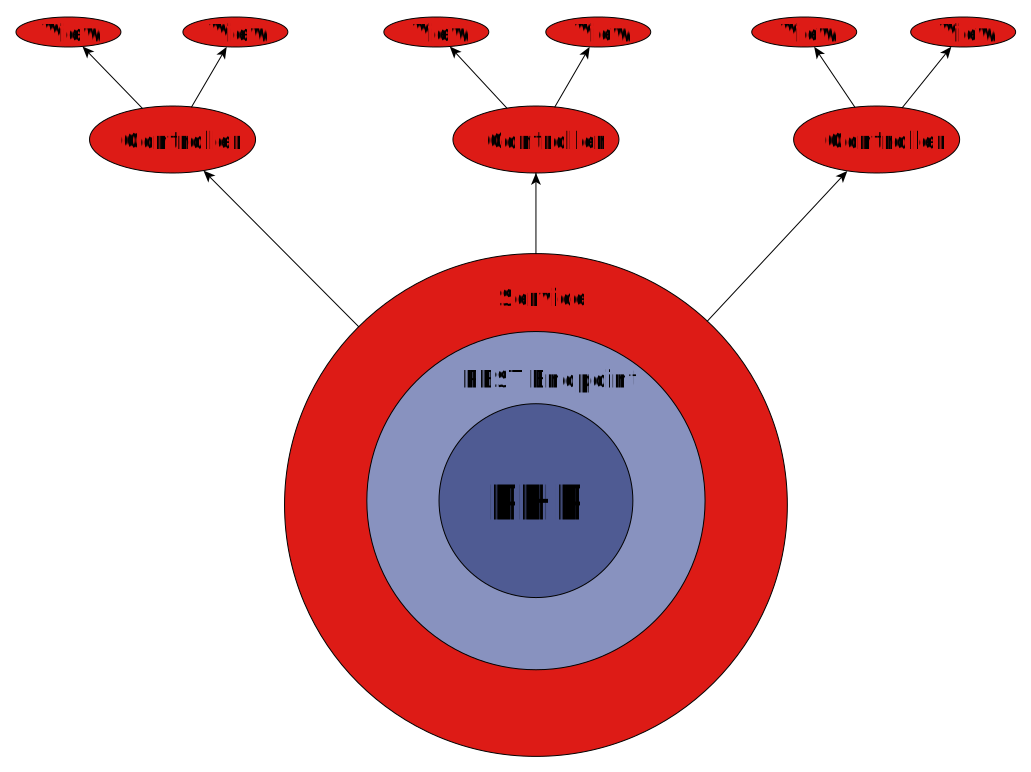
\includegraphics[scale=0.25]{../artifacts/angular-architecture.pdf}
\caption{Angular Architecture}
\label{fig:angular-architecture}
\end{figure}
\end{frame}

\subsection{REST}
\begin{frame}
\frametitle{Representational State Transfer (REST)}
\begin{defn}
\textbf{REST}, a mnemonic for \textbf{Representational State Transfer}, is a software architectural pattern that lays out how to interchange data amongst different sites.
\end{defn}

\mbox{}\\
REST allows sites with different backends, different languages, different use cases, etc. to easily exchange information without the complication of writing site-to-site specific integration code. REST rides on top of standard HTTP verbs to perform a standard set of operations. Using the ubiquity of HTTP, REST is an easy-to-program, agreed upon standard for exchanging data among sites.
\end{frame}

\subsection{Promises}
\begin{frame}
\frametitle{Promises}
\begin{defn}
A \textbf{promise} is a service that helps one run a method asynchronously and use the return values (or exceptions) when they are available.
\end{defn}

\mbox{}\\
A promise can be thought of as a ``latent if'' that allows for asynchronous operations to process as they happen. \cite{promise} For instance, suppose a HTTP request is made to an external API. The promise will \textbf{wait} and inform Angular of three possible outcomes:
\begin{enumerate}
	\item \label{enum:accept}\textbf{Successful Contact \& Data:} Data was returned successfully
	\item \label{enum:no-data}\textbf{Successful Contact, Failure on Data:} The server had no data
	\item \label{enum:bad-kitty}\textbf{Completely Unsuccessful:} The server was offline
\end{enumerate}
In case \ref{enum:accept}, the promise is \textbf{accepted}. Cases \ref{enum:no-data} \& \ref{enum:bad-kitty} are \textbf{rejected}.
\end{frame}

\section{Angular Components}
\subsection{Services}
\begin{frame}
\frametitle{Services}
\begin{defn}
A \textbf{service} is a layer that rides on an asynchronous operation (e.g., a REST API endpoint) that uses a promise to handle the latency and results.
\end{defn}

A service acts as a bridge from an asynchronous operation to a promise object, where it can processed and interpreted by controllers. Services are normally a REST API endpoint, but can be any asynchronous event, such as a click event, an exception, a redirect, or a timer. All services will have the following properties:
\begin{itemize}
	\item \textbf{Input:} Parameter(s) needed to fire up the service
	\item \textbf{Output:} Promise containing the results when they are ready
\end{itemize}

Services standardize asynchronous events such as AJAX and DOM events and provide a common API to handle them.
\end{frame}

\subsection{Controllers}
\begin{frame}
\frametitle{Controllers}
Controllers are the focal point for Angular development. The definition is identical as from the MVC design pattern. Each controller is \emph{dependency injected} with the services and other dependencies it requires.

\begin{defn}
\textbf{Dependency Injection} is a design pattern in which a dependent object is dynamically injected into an object's state variables.
\end{defn}

Dependency Injection is the center of Angular's flexibility: what one object needs can be determined on an individual case-by-case basis by the developer and dynamically loaded and instantiated by Angular on demand. This way, only the objects needed are loaded--no more, no less. Dependency Injection is a main feature of Angular, and has been a core feature of software frameworks such as Java Spring for many years. \cite{dependency-injection, spring}
\end{frame}

\begin{frame}
\frametitle{Using Controllers}
Once dependencies have been (easily) resolved via dependency injection, controllers act as the main hub for data flowing to and from the backend. A controller can consist of anything the developer can imagine. From a pragmatic standpoint, controllers normally utilizes \texttt{\$scope}, which contains the state of the controller. \texttt{\$scope} largely consists of two items:

\begin{enumerate}
	\item \textbf{state variables:} state variables, many of which have been loaded after accepting or rejecting a promise from a service
	\item \textbf{methods:} methods that respond to promises, user input, and other DOM events
\end{enumerate}

Using these two items, controllers act as the bridge from the backend to the frontend.
\end{frame}

\subsection{Directives}
\begin{frame}
\frametitle{Directives}
\begin{defn}
A \textbf{directive} is an Angularific marker in the DOM that uses custom HTML to inject an Angular customized behavior on the DOM. 
\end{defn}
The main idea of a directive is to define a generalized behavior and inject it as necessary using standard HTML syntax. \cite{directives} Directives can be custom HTML attributes, tags, classes, or comments. Angular has many predefined directives:

\begin{itemize}
	\item \textbf{ng-class:} Use a class if a condition is true.
	\item \textbf{ng-repeat:} Loop through an array in \texttt{\$scope}, \textbf{foreach} style.
	\item \textbf{ng-show:} Show if a condition is true.
\end{itemize}

The power of directives is that one can specify directives to inject anything into the DOM, \texttt{\$scope}, etc.
\end{frame}

\subsection{Angular Bootstrap}
\begin{frame}
\frametitle{Angular Bootstrap}
The \textbf{Angular Bootstrap} project provides a freely available set of directives that allow one to use Bootstrap's JavaScript components using Angular. Standard Bootstrap uses jQuery to drive its JavaScript components. Angular Bootstrap isolates the jQuery dependent components and eliminates the requirement to include jQuery or Bootstrap's JavaScript files. The components available include:

\begin{itemize}
	\item Carousels
	\item Drop Down Menus
	\item Modals
	\item Typeaheads
\end{itemize}

\dots and more. \cite{angular-bootstrap}
\end{frame}

\begin{frame}[allowframebreaks]
\frametitle{Works Cited}
\bibliography{angular}
\end{frame}

\end{document}